\documentclass[conference]{IEEEtran}
\usepackage{times}
\usepackage{amsmath}
\usepackage{amsfonts}
% numbers option provides compact numerical references in the text.
\usepackage[numbers]{natbib}
\usepackage{multicol}
\usepackage[bookmarks=true]{hyperref}
\usepackage{balance}
\usepackage{graphics} % for pdf, bitmapped graphics files
\usepackage{graphicx}
\usepackage{epsfig} % for postscript graphics files
\usepackage{color}



\newtheorem{theorem}{Theorem}
\newtheorem{proposition}{Proposition}
\newtheorem{lemma}{Lemma}

\pdfinfo{
   /Author (Homer Simpson)
   /Title  (Robots: Our new overlords)
   /CreationDate (D:20101201120000)
   /Subject (Robots)
   /Keywords (Robots;Overlords)
}

\begin{document}

% paper title
\title{Decentralized Ergodic Control: Multi-Agent Something}

% You will get a Paper-ID when submitting a pdf file to the conference system
\author{Author Names Omitted for Anonymous Review. Paper-ID [add your ID here]}

%\author{\authorblockN{Michael Shell}
%\authorblockA{School of Electrical and\\Computer Engineering\\
%Georgia Institute of Technology\\
%Atlanta, Georgia 30332--0250\\
%Email: mshell@ece.gatech.edu}
%\and
%\authorblockN{Homer Simpson}
%\authorblockA{Twentieth Century Fox\\
%Springfield, USA\\
%Email: homer@thesimpsons.com}
%\and
%\authorblockN{James Kirk\\ and Montgomery Scott}
%\authorblockA{Starfleet Academy\\
%San Francisco, California 96678-2391\\
%Telephone: (800) 555--1212\\
%Fax: (888) 555--1212}}


% avoiding spaces at the end of the author lines is not a problem with
% conference papers because we don't use \thanks or \IEEEmembership


% for over three affiliations, or if they all won't fit within the width
% of the page, use this alternative format:
%
%\author{\authorblockN{Michael Shell\authorrefmark{1},
%Homer Simpson\authorrefmark{2},
%James Kirk\authorrefmark{3},
%Montgomery Scott\authorrefmark{3} and
%Eldon Tyrell\authorrefmark{4}}
%\authorblockA{\authorrefmark{1}School of Electrical and Computer Engineering\\
%Georgia Institute of Technology,
%Atlanta, Georgia 30332--0250\\ Email: mshell@ece.gatech.edu}
%\authorblockA{\authorrefmark{2}Twentieth Century Fox, Springfield, USA\\
%Email: homer@thesimpsons.com}
%\authorblockA{\authorrefmark{3}Starfleet Academy, San Francisco, California 96678-2391\\
%Telephone: (800) 555--1212, Fax: (888) 555--1212}
%\authorblockA{\authorrefmark{4}Tyrell Inc., 123 Replicant Street, Los Angeles, California 90210--4321}}


\maketitle

\begin{abstract}
    This work is presented in two parts.
    In the first part, we formulate the pursuit-evader problem as a probabilistic problem for robotic agents with sensors.
    An ergodic control policy is derived for the nonlinear dynamics of the robotic agent.
    We show that this ergodic control policy is optimal for both the pursuer and the evader.
    In the second part of this work, we reformulate the ergodic controller in a decentralized manner.
    Using methods found in multi-agent consensus, we show that the decentralized controller is equivalent to the centralized case.
    Last, we show that this decentralized control policy can be extended to other problems such as mapping and estimation.
\end{abstract}

\IEEEpeerreviewmaketitle

\section{Introduction}

The pursuit-evasion problem is an active area of research where the goal for the pursuer is to localize the evader and the goal of the evader is to be as far away from the pursuer~\citet{++}.
Many solutions to this problem exists within game theory~\citet{++} where specific strategies are shown to have equilibrium properties where both the pursuer and evader can adopt optimal policies where no one is at an advantage.
Other solutions exist within the field of optimal control~\citet{++}.
Here, the problem is often specified as extremizing an objective function subject to dynamic and control constraints.
Similarly, the concept of equilibrium solutions play a role for finding the best possible policy that the pursuer and evader can adopt.
However, much of the work fails to consider a robotic agent's dynamics as well as the sensor dynamics for which the robot senses it's environment.
Such control strategies have been developed to localize targets as well as map environments, but do not consider the pursuit-evasion problem, nor the capabilities of these solutions to be equilibrium solutions.

Pursuit-evasion game as it is known in some literature~\cite{++}, is defined with at least two autonomous agents, a pursuer and an evader.
The goal of the pursuer is to localize the evader's position, whereas the evader's goal is the opposite.
Often this is represented in optimal control as a minimization or a maximization problem of the distance of the pursuer to the evader~\cite{++}. 
In other instances, the pursuit-evasion game is defined over a finite grid of positions where the pursuer and the agent are allowed to move within. 
Both agents are capable of making finite actions that move them from one grid point to the next sequential grid point.
Other work defined the problem as a Markov Decision Process (MDP). 
In the MDP formulation, the agents move about a graph dictated by the state transition probabilities~\cite{++} and the resulting actions that enable the agents to arrive at their current state.

Current advances in active sensing and exploration consider the probabilistic nature of localization tasks subject to sensor dynamics~\cite{miller2016ergodic, miller2015optimalrange,ansari2016sequential}.
Moreover, specifying the problem as an ergodic coverage problem allows both the flexibility of the choice of objective function, and enables solving coverage of non-convex probabilistic distribution.
Specifically, the mentioned work solves localization problems by considering the sensor dynamics and where the sensor readings are most informative about the target's location.

In this paper, we contribute a formulation of an ergodic control policy as a solution to the pursuit-evader problem.
The formulation considers a hybrid control switching approach where control actions are not necessarily considered optimal controls, but rather improvements to the ergodic objective subject to a user-specified existing default control policy.
By iterating on this policy, we show consistent decrease in the objective function and an improvement in the estimate of the task.
We then contribute a decentralized formulation of the same controller for use in multi-agent ergodic control.
The pursuit-evader problem is presented for the decentralized multi-agents.
We solve that problem as well.
As it turns out, this control policy works for other problems such as mapping and estimating terrain.

The paper is outlined as: Section \ref{sec:ergcontrol} formulates the ergodic control problem for the pursuit-evader problem.
Section~\ref{sec:decentralized}
Section \ref{sec:est} extends the ergodic control formulation for problems in exploration, estimation and localization.
Last, Section~\ref{sec:conc} concludes the work.

\section{Ergodic Control as a Solution to Pursuit-Evasion} \label{sec:ergcontrol}

In this section, we define an ergodic control policy for the pursuit-evasion game. 
We first define the pursuit-evasion game in a probabilistic setting where the location of the evader is defined as a probability function given measurements from bearing only sensors from the pursuers. 
We then define information measures of where the sensor is most likely to provide the most informative measurements about the evader.
Next we derive the ergodic control policy using hybrid systems theory. 
Last, we show how the specification of the pursuit-evasion game as an ergodic control problem has a Nash equilibrium solution and how this is broken based on specific advantages that the pursuer or the evader may have.

\subsection{Pursuit-Evasion Problem Statement}

In this work, we define the state of the pursuer and evader agents as $x_p(t), x_e(t) \in \mathbb{R}^n$ respectively.
The agent's motion is then defined as a control-affine dynamical system of the form
\begin{equation}
\dot{x} = f(x,u) = g(x) + h(x)u
\end{equation}
where $u \in \mathbb{R}^m$ is the control action, $g(x) : \mathbb{R}^n \to \mathbb{R}^n$ is the free dynamics, and $h(x) : \mathbb{R}^n \to \mathbb{R}^{n \times m}$ as the control vectors. 
We also define a sensor model $\Upsilon(x_p, x_e): \mathbb{R}^n \times \mathbb{R}^n \to  \mathbb{R}^p$ where sensor measurements are given as $y = \Upsilon(x_p, x_e) \in \mathbb{R}^p$.
The goal of the pursuer will then be to determine the position of the evader to some $\epsilon$ given the history of measurements, or
\begin{equation}
p( x_e \mid y_i, x_{p,i}) 
\end{equation}





\subsection{Ergodic Metric}

Consider a robot whose state is defined as $x \in \mathbb{R}^n$ and the control input to the robot is $u \in \mathbb{R}^m$.
The time evolution of the robot is then assumed to be governed by the control-affine dynamical system of the form
\begin{equation} \label{eq:robot_dynamics}
\dot{x} = f(x,u) = g(x) + h(x) u
\end{equation}
where $g(x) : \mathbb{R}^n \to \mathbb{R}^n$ is the free dynamic response of the robot, and $h(x): \mathbb{R}^n \to \mathbb{R}^{n \times m}$ is the driving dynamic response subject to input $u$.
Next, let us define a bounded domain $\mathcal{X}_v \subset \mathbb{R}^v$  whose limits are $\left[0,L_1 \right] \times \left[ 0,L_2 \right] \times \ldots \left[ 0, L_v\right]$ with $v\le n$. 
The time-averaged statistics $c(s, x(t))$ of the robot's trajectory $x(t)$ (i.e., where the robot spends most of its time) for some time interval $t \in \left[ t_i, t_i + T\right]$ by
\begin{equation}
c(s, x(t)) = \frac{1}{T}\int_{t_i}^{t_i+T} \delta (s - x(t)) dt
\end{equation}
where $\delta$ is a Dirac delta function, $T \in \mathbb{R}^+$ is the time horizon, $t_i \in \mathbb{R}^+$ is the $i^\text{th}$ sampling time, and $s \in \mathbb{R}^v$ is the search domain.
We then define a ``target'' distribution $\phi(s) : \mathcal{X}_v \to \mathbb{R}^+$ with which the robot agent is to be ergodic with respect to (i.e., time spent during a trajectory $x(t)$ is proportionate to the spatial statistics of that region).
The ergodic metric which relates the two distributions $c(s,x(t))$ and $\phi(s)$ is:
\begin{align} \label{eq:ergodic_metric}
\mathcal{E}(x(t)) & = q \,\sum_{k \in \mathbb{N}^v} \Lambda_k \left(c_k -\phi_k \right)^2   \\
& = q \, \sum_{k \in \mathbb{N}^v} \left( \frac{1}{T} \int_{t_i}^{t_i + T} F_k(x(t)) dt - \int_{\mathcal{X}_v} \phi(s) F_k(s) ds \right)^2 \nonumber
\end{align}
where $c_k$ and $\phi_k$ are the Fourier decompositions\footnote{The cosine basis function is used, however, any choice of basis function $F_k$ can be used.} of $c(s,x(t))$ and $\phi(s)$ with
\begin{equation*}
F_k(x) = \frac{1}{h_k}\prod_{i=1}^v \cos \left( \frac{k_i \pi x_i}{L_i} \right)
\end{equation*}
being the cosine basis function for a given coefficient $k \in \mathbb{N}^v$,  $h_k$ is the normalization factor defined in~\cite{mathew2011metrics}, and $\Lambda_k = (1 + \Vert k \Vert^2)^{-\frac{v+1}{2}}$ is a weight on the frequency coefficients.
Equation (\ref{eq:ergodic_metric}) now relates the time spent by the robot to the spatial statistics.
A robot whose control inputs result in a trajectory $x(t)$ that minimizes (\ref{eq:ergodic_metric}) is then said to be ergodic with respect to the target distribution.

Because we are computing the ergodic control in a receding horizon approach, and the target distribution $\phi(s)$ can be time-varying, a history of where the robot has been is maintained in memory in order to compute the ergodic metric.
The ergodic metric is then computed  by adding a time parameter $\Delta t_\mathcal{E}$ which governs how far into the past the robot must remember where it has been. 
Equation (\ref{eq:ergodic_metric}) then becomes
\begin{equation*}
\mathcal{E}(x(t)) = q \, \sum_{k \in \mathbb{N}^v} \left( \frac{1}{T} \int_{t_i-{\color{blue}\Delta t_\mathcal{E}} }^{t_i + T} F_k(x(t)) dt - \phi_k\right) ^2.
\end{equation*}


\subsection{Ergodic Control}

Control inputs that result in an ergodic robot with respect to a target distribution are synthesized using hybrid systems theory.
Instead of directly minimizing (\ref{eq:ergodic_metric}) with respect to $x(t)$ and $u$, we consider the sensitivity of (\ref{eq:ergodic_metric}) with respect to an infinitesimal application duration $\lambda \to 0$ of the best possible control $u_\star \in \mathbb{R}^m$ that sufficiently reduces (\ref{eq:ergodic_metric}) at time $\tau$ from some default control $u_\text{def} \in \mathbb{R}^m$.
Taking the derivative of (\ref{eq:ergodic_metric}) with respect to the duration $\lambda$ gives this sensitivity (known as the mode insertion gradient~\cite{vasudevan2013consistent, axelsson2008gradient, egerstedt2006transition,caldwell2016projection})
\begin{theorem}
The first order sensitivity of (\ref{eq:ergodic_metric}) (or mode insertion gradient) with respect to the control duration $\lambda$ of the applied control $u_\star(\tau)$ is given as
\begin{equation}
\frac{\partial \mathcal{E}}{\partial \lambda} \Big \vert_\tau = \rho(\tau)^T (f_2(\tau, \tau) - f_1(\tau))
\end{equation}
where $f_2(t, \tau) = f(x(t), u_\star(\tau))$, $f_1(t) = f(x(t), u_\text{def}(t))$, and $\rho \in \mathbb{R}^n$ is the adjoint variable which is the solution to the backwards differential equation
\begin{equation}
\dot{\rho} = - 2 \frac{q}{T} \sum_{k \in \mathbb{N}^v} \Lambda_k (c_k - \phi_k) \frac{\partial F_k}{\partial x} - \frac{\partial f}{\partial x}^T \rho
\end{equation}
where $\rho(t_i + T) = \bold{0} \in \mathbb{R}^n$.
\end{theorem}
\begin{proof}
Taking the derivative of (\ref{eq:ergodic_metric}) with respect to $\lambda$ gives us
\begin{align}\label{eq:mode_insertion1}
\frac{\partial \mathcal{E}}{\partial \lambda} & = 2 \frac{q}{T}\sum_{k \in \mathbb{N}^v} \Lambda_k(c_k - \phi_k)\frac{\partial}{\partial \lambda} \int_{\tau}^{t_0+T} F_k(x(t))dt \\
& =2 \frac{q}{T}\sum_{k \in \mathbb{N}^v} \Lambda_k(c_k - \phi_k) \int_{\tau}^{t_0+T} \frac{ \partial F_k(x(t))}{\partial x} \frac{\partial x(t)}{\partial \lambda}dt. \nonumber
\end{align}
From~\cite{mode transition stuff} and the fact that
\begin{equation}
\frac{\partial x(t)}{\partial \lambda} = \Phi(t,\tau) \left( f_2(\tau, \tau) - f_1(\tau) \right),
\end{equation}
and $\Phi(t, \tau)$ is the state transition matrix, (\ref{eq:mode_insertion1}) is written as
\begin{equation} \label{eq:mode_intersion2}
\frac{\partial \mathcal{E}}{\partial \lambda} = \rho(\tau)^T \left( f_2(\tau, \tau) - f_1(\tau) \right),
\end{equation}
where  
\begin{equation} \label{eq:adjoint1}
\rho(\tau) = 2 \frac{q}{T}\sum_{k \in \mathbb{N}^v} \Lambda_k(c_k - \phi_k) \int_{\tau}^{t_0+T} \frac{ \partial F_k(x(t))}{\partial x} \Phi(t,\tau)dt.
\end{equation} 
We can see that (\ref{eq:adjoint1}) is a convolution equation for
\begin{equation}
\dot{\bold{\rho}} = - 2\frac{q}{T}\sum_{k \in \mathbb{N}^v}\Lambda_k(c_k - \phi_k) \frac{\partial F_k(x)}{\partial x} - \frac{\partial f}{\partial x }^T \rho
\end{equation}
where $\rho \in \mathbb{R}^n$, $\rho(t_0+T) = \bold{0} \in \mathbb{R}^n$.
Thus, the mode insertion gradient is given as
\begin{equation}
 \frac{\partial \mathcal{E}}{\partial \lambda}\Big | _\tau = \rho(\tau) ^T (f_2(\tau,\tau) - f_1(\tau))
\end{equation}
subject to
\begin{equation}
\dot{\bold{\rho}} = - 2\frac{q}{T}\sum_{k \in \mathbb{N}^v}\Lambda_k(c_k - \phi_k) \frac{\partial F_k(x)}{\partial x} - \frac{\partial f}{\partial x }^T \rho.
\end{equation}
\end{proof}

Given the mode insertion gradient, we aim to find the control $u_\star$ that provides the most significant decrease in the objective (\ref{eq:ergodic_metric}).
To do so, we define a secondary objective function 
\begin{equation}\label{eq:secondary_objective}
J_2 = \int_{t_i}^{t_i + T} \frac{\partial \mathcal{E}}{\partial \lambda} + \frac{1}{2}\Vert u_\star - u_\text{def} \Vert_R^2
\end{equation}
where $R \in \mathbb{R}^{m \times m}$ is a positive definite matrix which weighs $u_\star$.
\begin{proposition}
The solution to $u_\star$ that minimizes (\ref{eq:secondary_objective}) is given as
\begin{equation} \label{eq:ustar}
u_\star(t) = -R^{-1} h(x)^T \rho(t) + u_\text{def}(t)
\end{equation}
\end{proposition}
\begin{proof}
Taking the derivative of (\ref{eq:secondary_objective}) with respect to control $u_\star$ and setting the solution to zeros gives
\begin{align}\label{eq:secondary_objective2}
\frac{\partial J_2}{\partial u_\star} & = \int_{t_i}^{t_i + T} \frac{\partial }{\partial u_\star} \left( \frac{\partial \mathcal{E}}{\partial \lambda}\right) + R(u_\star - u_\text{def}) dt \nonumber \\
& = \int_{t_i}^{t_i + T}  h(x)^T\rho + R(u_\star - u_\text{def}) dt = 0.
\end{align}
Solving for $u_\star$ in (\ref{eq:secondary_objective2}) gives
\begin{equation}
u_\star = -R^{-1}h(x)^T\rho + u_\text{def}
\end{equation}
\end{proof}
\begin{theorem}
Assuming that $h(x)^T \rho \neq 0$, the mode insertion gradient in (\ref{eq:mode_insertion}) is always negative for $u_\star$ defined in (\ref{eq:ustar}), that is $\frac{\partial \mathcal{E}}{\partial \lambda} < 0 \forall u_\star \in \mathcal{U}$ where $\mathcal{U}$ is the control space.
\end{theorem}
\begin{proof}
Inserting (\ref{eq:ustar}) into (\ref{eq:mode_insertion}) gives
\begin{align}\label{eq:mode_insertion_neg}
\frac{\partial \mathcal{E}}{\partial \lambda} &= h(x)^T\rho \left(-R^{-1} h(x)^T\rho \right) \nonumber \\
& = -\rho^Th(x)R^{-1}h^T\rho = - \Vert h(x)^T\rho \Vert_{R^{-1}}^2 < 0.
\end{align}
Thus (\ref{eq:mode_insertion_neg}) shows us that $\forall u_\star \in \mathcal{U}$ defined in (\ref{eq:ustar}), $\frac{\partial \mathcal{E}}{\partial \lambda}<0$.
\end{proof}
Proving that (\ref{eq:ustar}) always provides a negative $\frac{\partial \mathcal{E}}{\partial \lambda}$ suggests that each control that is chosen will result in a decrease in (\ref{eq:ergodic_metric}) thus eventually minimizing the ergodic metric.

In robotics it is necessary to saturate the resulting control due to actuation limits in the robot. 
However, we still need to ensure that the resulting saturated control still results in a decrease in the objective function.
In this work, we select a time of application $\tau$ that results in the most negative mode insertion gradient, or more formally written
\begin{equation*}
\tau_\star= \underset{\tau}{\text{argmin }} \frac{\partial \mathcal{E}}{\partial \lambda}.
\end{equation*}
A line search~\cite{armijo1966minimization} is then used to find the duration $\lambda$ that significantly reduces (\ref{eq:ergodic_metric}) subject to the saturated control $u_\star(\tau)$.
The resulting control is then added to the default control $u_\text{def}(t) = u_\star(\tau) \forall t \in \left[ \tau-\lambda/2, \tau+\lambda/2 \right] \cap \left[ t_i, t_i+t_s\right]$ where $t_s$ is the sampling time and $u_\star(\tau)$ is saturated.

\subsection{Target Distribution}

For the pursuit-evasion problem, we specify the target distribution for the pursuer as 
\begin{equation}
\phi(s) = \eta \det \left[ \int_{x_e} I(s, x_e) p(x_e) dx_e \right]
\end{equation}
where 
\begin{equation}
I(x,x_e) =  \frac{\partial \Gamma(s, x_e)}{\partial x_e}^T \Sigma^{-1} \frac{\partial \Gamma(s, x_e)}{\partial x_e}
\end{equation}
is the Fisher Information Matrix~\cite{++} and $\eta$ is a normalization factor.
The target distribution for the evader is then set as 
\begin{equation}
\phi(s) = 1 - \eta \det \left[ \int_{x_e} I (x_p, s) p(x_e) dx_e\right].
\end{equation}
We assume that the estimate of the location of the evader is known to both the evader and the pursuer. 
As a result, the pursuer will be ergodic with respect to the regions where information about the evader is highest given the Fisher information of the sensor model. 
The evader is then ergodic with respect to the where information is least informative about itself given the sensor model of the pursuer. 

\subsection{Decentralized Ergodic Control}

Consider the $N$ multi-agent robotic dynamics 
\begin{align}
\dot{x} = f(x, u) &= g(x) + h(x)u \\
& =  \begin{bmatrix}
g_1(x_1) \\
g_2(x_2) \\
\vdots \\
g_{N}(x_N)
\end{bmatrix}
+ \begin{bmatrix}
h_1(x_1) \\
h_2(x_2) \\
\vdots \\
h_{N}(x_N)
\end{bmatrix}u.
\end{align}
Assuming that knowledge of where the robot has been and will go is known, the contribution of each agent to the Fourier decomposition of the time-averaged statistics $c_k$ of the multi-agent system can be written as
\begin{equation}
c_k = \frac{1}{N} \sum_{j=1}^{N} \frac{1}{T} \int_{t_i - \Delta t_\mathcal{E}}^{t_i+T} F_k(x_j(t))dt.
\end{equation}

The derivation of the decentralized ergodic control problem first assumes that there exists an underlying connected network for which each agent can communicate with one another. Assume that the connections can be represented via a graph Laplacian $L$ \cite{deo2016graph}. A consensus matrix $P$ can be generated from the graph Laplacian such that $P$ is both row and column stochastic \cite{deo2016graph, bertsekas1989parallel}. In the decentralized case, the ergodic metric is defined as
%\begin{equation}
%\mathcal{E}_i(x_i(t)) = \sum_{k \in \mathbb{Z}} (\phi_k - \sum_j (P \otimes I_{\vert k \vert})_{ij} c_{k,j})^2
% \end{equation}
 \begin{equation} \label{eq:derg}
\mathcal{E}_i(x_i(t)) = \sum_{k \in \mathbb{Z}} (\phi_k - \sum_j P_{ij} c_{k,j})^2
 \end{equation}
for each agent $i$ with neighbors $j$. The consensus matrix $P$ is used to transmit information about where each agent has explored (and is going to explore) to neighboring agent. As a result of sharing this information, each agent is able to synthesize a control solution that is sensitive to what the network of agents has explored. Hence, consensus improves exploration efficiency for the overall network. 
\begin{lemma}

\end{lemma}

Following the derivation of the centralized ergodic controller, the mode insertion gradient for an individual agent is then,
\begin{equation*}
\frac{d \mathcal{E}_i}{d \lambda} = \rho_i(s) (f_i(x_i(s), u_{2,i}(s)) - f_i(x_i(s), u_{1,i}(s)))
\end{equation*}
with the costate equation obtained from the backwards-differential equation
%\begin{equation}
%\dot{\rho}_i = - \sum_{k \in \mathcal{Z}}(\phi_k - \sum_j (P \otimes I_{\vert k \vert})_{ij} c_{k,j}) \frac{\partial F_{k,i}(x_i)}{\partial x_i} - \frac{\partial f_i}{\partial x_i }^T \rho_i.
%\end{equation}
\begin{equation*}
\dot{\rho}_i = - \sum_{k \in \mathcal{Z}}(\phi_k - \sum_j P _{ij} c_{k,j}) \frac{\partial F_{k,i}(x_i)}{\partial x_i} - \frac{\partial f_i}{\partial x_i }^T \rho_i.
\end{equation*}
The solution to the secondary cost function for an individual agent
\begin{equation*}
J_{2,i} = \frac{d \mathcal{E}_i}{d \lambda} + \frac{1}{2} \Vert u_{2,i} - u_{1,i}\Vert ^2_{R_i}
\end{equation*}
is
\begin{equation}
u^*_i(t) = -R_i^{-1} h_i(x_i)^T \rho_i(t) + u_{1,i}(t)
\end{equation}
which is equivalent to the individual agent's control solution as the stacked representation of the centralized case (\ref{eq:central}). Individual time of control application $\lambda$ can be found with
\begin{equation*}
\lambda ^*= \underset{\lambda}{\text{argmin }} \frac{d\mathcal{E}_i (\lambda)}{d\lambda} .
\end{equation*}
%However, the time of action of one agent may interfere with another agent, impeding on reduction of the ergodic metric. This can be solved by having a consensus on the first order sensitivity of control application and finding the time of application that achieves the largest decrease in the ergodic metric. This can be written as
%\begin{equation}
%\lambda ^*= \underset{\lambda}{\text{argmin }} N\sum_j P_{ij} \frac{d \mathcal{E}_j (\lambda)}{d\lambda}
%\end{equation}
%and is equivalent to finding the time of control application in the centralized ergodic control formulation.

\begin{theorem}
For a connected network of agents with control-affine dynamics (\ref{eq:caff}), the decentralized ergodic control problem (\ref{eq:derg}) is equivalent to the centralized ergodic control problem (\ref{eq:cerg}) when a consensus on the $c_{k,i}$ values is reached.
\end{theorem}
{\it Proof: } Assume there exists a consensus matrix $P$ that is row and column stochastic and described a connected graph. The operation $ \sum_j P_{ij} c_{k,j}$ is equivalent to taking an average of the local $c_k$ values for each neighboring agent $j$. Thus, we can rewrite the consensus on $c_k$ as
%\begin{equation}
%\sum_j (P \otimes I_{\vert k \vert})_{ij} c_{k,j} = \frac{1}{N}\sum_j \frac{1}{T} \int_{t_0}^{t_0 +T} F_k(x_j(t)) dt.
%\end{equation}
\begin{equation}
\lim_{t_k \to \infty}\sum_j P_{ij}^{t_k} c_{k,j} = \frac{1}{N}\sum_j \frac{1}{T} \int_{t_0}^{t_0 +T} F_k(x_j(t)) dt.
\end{equation}
where $t_k$ is the number of times that the $P_{i,j} c_{k,j}$ values have been iterated upon. The summation over all neighboring agents can be brought into the integral to give
%\begin{equation}
%\begin{aligned}
% \sum_j (P \otimes I_{\vert k \vert})_{ij} c_{k,j} &=  \frac{1}{T} \int_{t_0}^{t_0 +T} \frac{1}{N}\sum_j F_k(x_j(t)) dt \\
%&= \frac{1}{T} \int_{t_0}^{t_0 +T} \tilde{F}_k(x(t)) dt
%\end{aligned}
%\end{equation}
\begin{equation}
\begin{aligned}
\lim_{t_k \to \infty}\sum_j P_{ij}^{t_k} c_{k,j} &=  \frac{1}{T} \int_{t_0}^{t_0 +T} \frac{1}{N}\sum_j F_k(x_j(t)) dt \\
&= \frac{1}{T} \int_{t_0}^{t_0 +T} \tilde{F}_k(x(t)) dt
\end{aligned}
\end{equation}
which when $t_k \to \infty$, a consensus is reached on where each agent has explored. Thus for any connected graph, the consensus is equivalent to (\ref{eq:ckn}).

Regardless of whether consensus amongst agents is reached, the ergodic measure for an individual agent will still be reduced asymptotically as $t \to \infty$. Consider that there exists a control action $u$ that minimizes the ergodic cost (\ref{eq:derg}). Then the mode insertion gradient (\ref{eq:mode_insert}) is $\le 0$ for some $u^*(\lambda)$ which defines the rate of reduction of the cost at time $\lambda$. As a result, any partial consensus will be included in the sensitivity of the ergodic metric with respect to neighboring agents' actions. Thus, consensus only impacts the rate of convergence of the ergodic metric and is dependent on the network connectivity.

\section{Network and Consensus} \label{sec:network}

In the previous section, we described the effects of consensus on the decentralized ergodic controller. In particular, the rate of convergence for both minimization of the ergodic metric and consensus on the $c_k$ values of each agent depend on the connectivity of the graph itself. In this section, we discuss the formulation of the consensus matrix $P$ that can be used for the decentralized ergodic controller.

\begin{figure}[th]
\centering
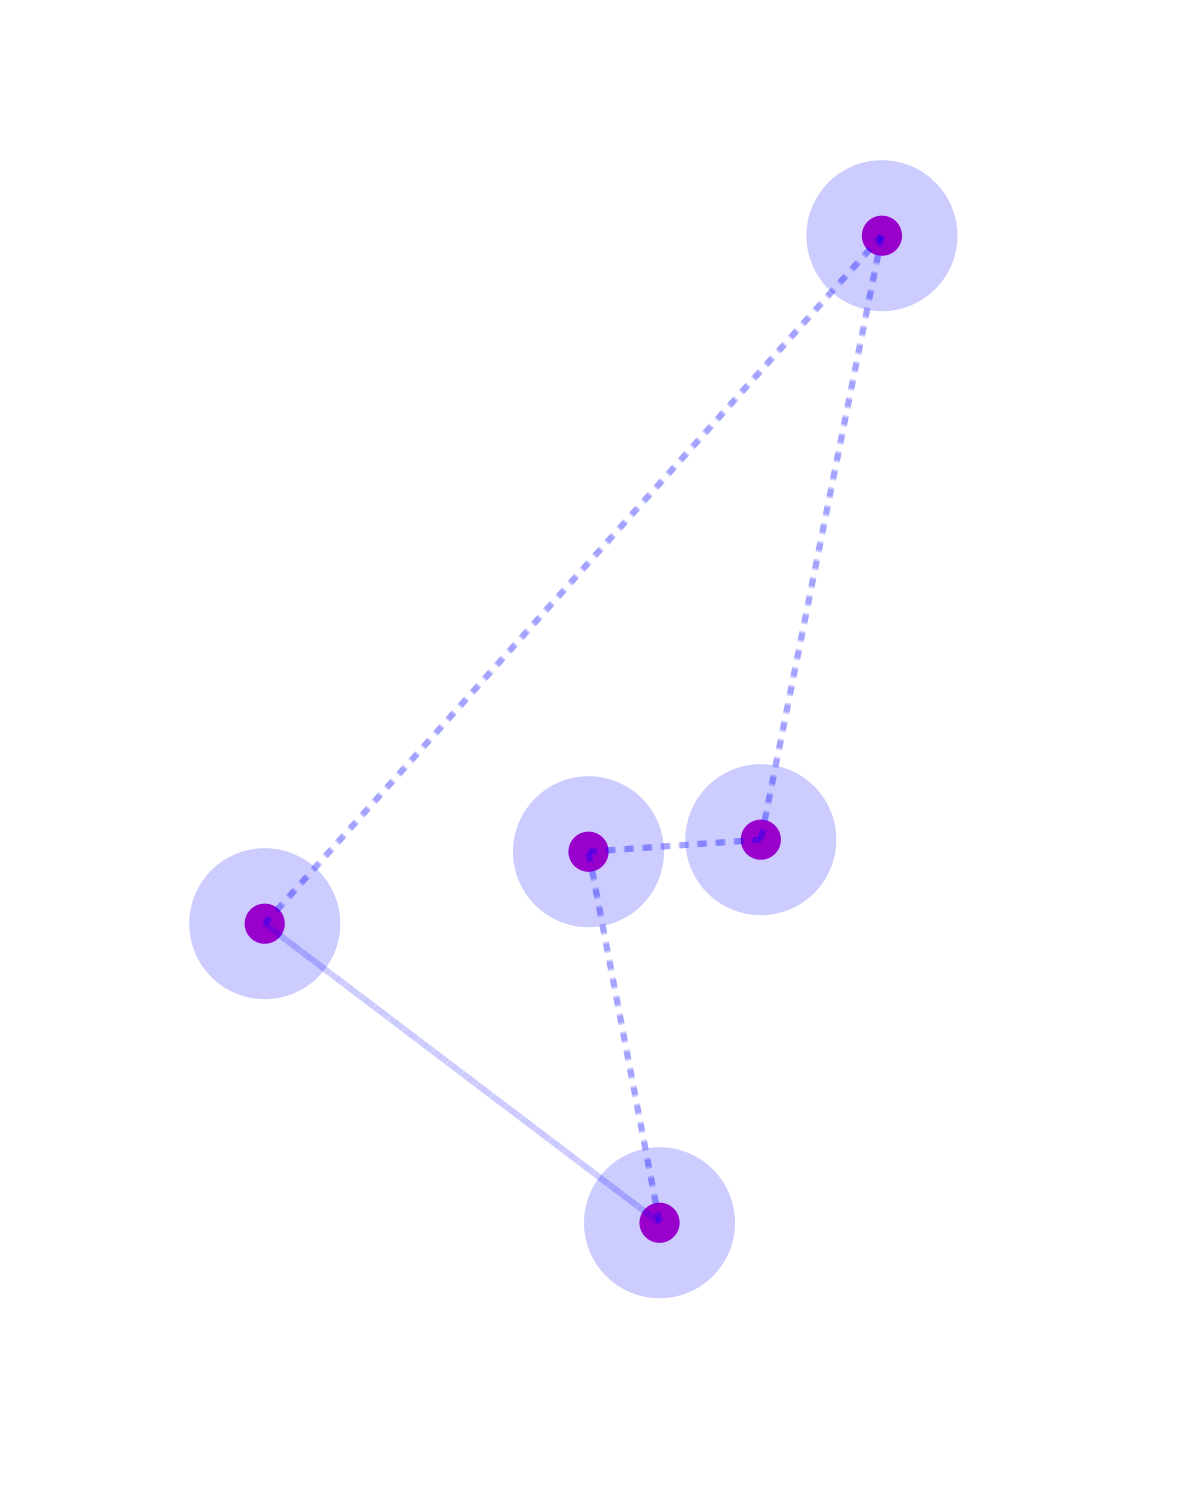
\includegraphics[scale=0.4]{figures/5networkpath.png}
\caption{ A ring network connection defined for a set of $n$ vertices with edges $(i,i+1) \cup (n,1)$ for $i \in \{1, \ldots, n\}$ is used for localization and estimation examples. The dotted lines represent the connection between each agent. Each agent is represented by the circle. }
\label{fig:path}
\end{figure}

For the decentralized ergodic controller, any consensus matrix can be designed so long as the consensus matrix is row and column stochastic. This implies that the resulting consensus matrix must approximate the average of all the agents' $c_k$ values. In an ideal situation where the graph is fully connected, consensus of the $c_k$ values will occur rapidly. However, as shown in the last section, even partial consensus will improve the rate of convergence of the ergodic metric. In a later discussion in the results, convergence of the ergodic measure is presented with a 1, 2, and 3 agent network with a complete graph topology. For the remainder of this work, a ring graph (see Fig.~\ref{fig:path}) is used as an arbitrary choice to show that the decentralized ergodic controller eventually reaches a consensus so long as the graph is connected. Future work will involve examining various consensus matrices and their effects on the rate of convergence of the ergodic metric.
\section{Estimation and Localization} \label{sec:est}

In this section we present a formulation of the decentralized ergodic control for estimation and localization problems. In general, problems of exploration for distributed information will take the same form as was developed initially in section~\ref{sec:network} where the spatial statistical distribution $\Phi$ is given.

\subsection{Estimation}

Typically estimation problems are formulated as a minimization of the sum of square errors of a set of measurement data $y_i$ taken at state $x_i \in \mathbb{R}^n$ and a prediction of the underlying measurement model that is likely to represent the data $\phi(\theta, x)$ where $\theta$ is some parameter that is to be estimated. Formally, the least-squares problem is described as
\begin{equation} \label{eq:leastSquares}
\begin{aligned}
& \underset{\theta}{\text{min}} \sum_{i}^{N} (y_i - \phi(\theta, x))^2
\end{aligned}
\end{equation}
Solutions to this problem exist in abundance \cite{marquardt1963algorithm, julier1997new, wan2000unscented}. There exists an equal abundance of work in estimation for distributed networks \cite{carli2008distributed, liu2014distributed, arablouei2014distributed}. In this work, we utilize a distributed Kalman filter \cite{carli2008distributed}, however any estimator which provides a statistical representation $p(\theta)$ over the set of parameters $\theta$ is sufficient for use in ergodic control. The only significant change in the ergodic control formulation is the target distribution $\Phi(x)$.

For an estimation problem, we utilize the expected information density (EID) of the estimator. The EID is first formulated with the definition of the Fisher information matrix given as
\begin{equation}
I(\theta, x) = \frac{\partial \phi(\theta, x)}{ \partial \theta} ^T \Sigma^{-1} \frac{\partial \phi(\theta, x)}{ \partial \theta}
\end{equation}
where $\Sigma^{-1}$ is the measurement covariance. The EID is then the expectation of information given the certainty of the estimated parameters, $p(\theta)$. That is, we define the EID as
\begin{equation}
\text{EID}(x) = \eta \int_\theta I(\theta, x) p(\theta) d\theta
\end{equation}
where $\eta$ is a normalization factor. For multi-parameter estimation, the determinant of the EID is defined as our target distribution $\Phi(x)$ which implies that each individual agent in the distributed network will have their own $\phi_k$ values given by
\begin{equation}
\phi_{k,i} = \int_X \text{det}\vert \text{EID}_i(x)\vert F_k(x) dx.
\end{equation}
However, consensus on each $\phi_{k,i}$ is not necessary as we are using estimators that form a consensus on the parameters $\theta$ and their statistical parameters \cite{carli2008distributed}. Thus, the only modification to the distributed ergodic control formulation is the need to recalculate $\phi_k$ whenever a new estimate of $\theta$ is provided. In this work, we use the example of mapping the terrain of a square domain region. Thus, measurements are considered to be local topological height.

\subsection{Target Localization}

Target localization is treated in the same manner as an estimation problem. Specifically, we are estimating the location of targets in the environment. In this work, we examine target localization in an environment filled with obstacles. A benefit of the formulation of ergodic control is the ease with which the objective function can be formulated. We assume that each robot has a map of the environment $\Gamma(x)$ that penalizes the robot if it is in collision with the obstacle. The primary objective function for each agent then becomes
\begin{equation}
\mathcal{E}_i(x_i(t)) = q_1\sum_{k \in \mathbb{Z}} (\phi_k - \sum_j P_{ij} c_{k,j})^2 + q_2\Gamma(x)
 \end{equation}
where the mode insertion gradient is
\begin{equation*}
\frac{d \mathcal{E}_i}{d \lambda} = \rho_i(s) (f_i(x_i(s), u_{2,i}(s)) - f_i(x_i(s), u_{1,i}(s)))
\end{equation*}
with the costate solved by the backwards differential equation
\begin{equation*}
\resizebox{0.5 \textwidth}{!}
{ $
\dot{\rho}_i = - 2 q_1\sum_{k \in \mathcal{Z}}(\phi_k - \sum_j P _{ij} c_{k,j}) \frac{\partial F_{k,i}(x_i)}{\partial x_i} - q_2\frac{\partial \Gamma(x_i)}{\partial x_i}- \frac{\partial f_i}{\partial x_i }^T \rho_i .
$
}
\end{equation*}
Thus, during forward trajectory prediction, the sensitivity will include future collisions that may occur.

Here, measurements $y_i$ are taken as global position measurements of the target relative to the world frame. Each robot will then have a sensor with a limited circular range $r$. Initially, none of the agents know the location of any of the targets, thus the EID is considered to be a uniform distribution.

The results for exploration, estimation, and target localization are shown in the following section.

\section{Results} \label{sec:res}

In this section, results are presented for three applications of decentralized ergodic control. The first example discusses the reduction of the ergodic measure during information-based exploration of a unknown distribution. In particular, we observe the effects of introducing agents in a complete graph network configuration (defined as a graph with $n$ vertices connected to all other vertices) and collaborative behavior amongst agents. The second example illustrates the improvement in area coverage for localizing targets in a crowded environment. The last example illustrates how the decentralized ergodic controller can be used for Fisher Information-based estimation of terrain topology.

\subsection{Information-Based Coverage}

Information-based exploration is presented with an example comparing coverage of a distribution using a 1, 2, and 3 agent network. The task for each agent is to maintain coverage of a distribution (see Fig.~\ref{fig:n_agent}) that is proportional to the information available (given by the heat map). This example is presented to illustrate the collaborative behavior of decentralized ergodic control when under consensus. Specifically, this collaborative behavior can be seen in the trajectory traces of the 2 and 3 agent network. Each agent covers one of the peaks of the distribution while the other spans the remaining peaks. The agents then trade off this behavior to get an improved reduction of the ergodic measure. The benefit of using a multi-agent distributed ergodic system is shown in the ergodicity measure in Fig.~\ref{fig:n_agent} where the rate of reduction in the ergodic metric increases with added agents.

\begin{figure}[ht!]
\centering
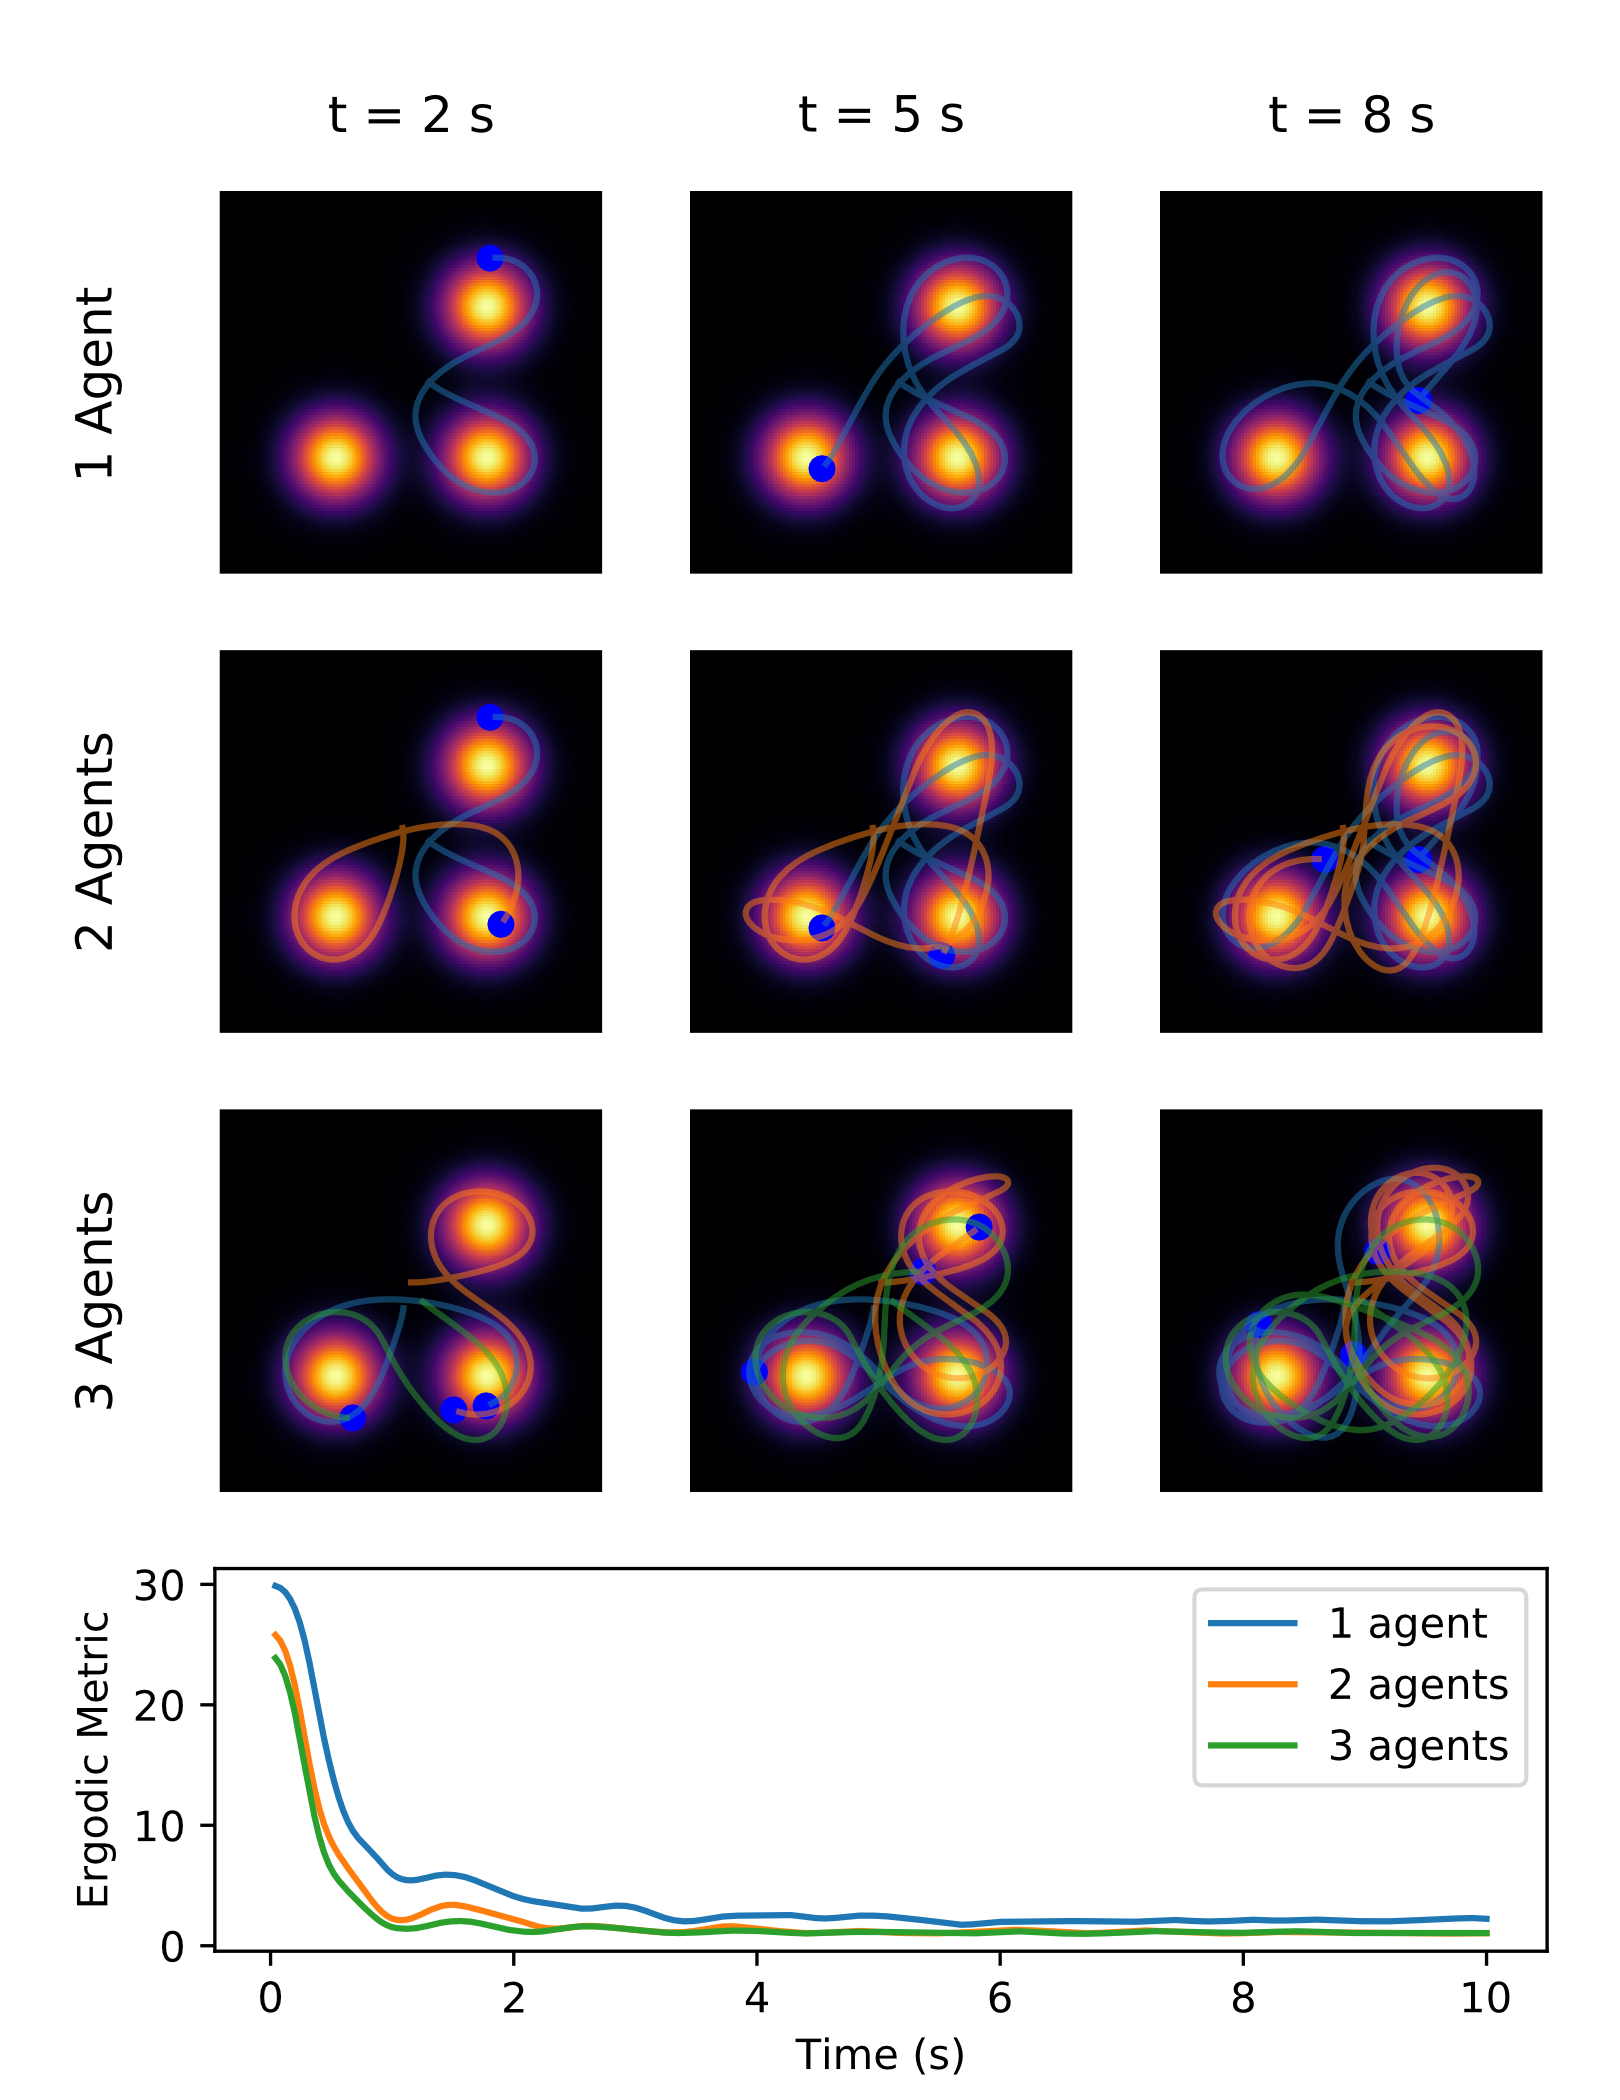
\includegraphics[scale=0.6]{figures/n_agent_comparison2.png}
\caption{ Information based exploration is shown with 1, 2, and 3 agents using ergodic control. Adding an additional agent automatically improves the coverage and reduction of the ergodic metric. Collaborative behavior is seen with the 2 and 3 agent systems where a trade-off occurs allowing a single agent to spend more time at a peak while the other agents span across the remaining information peaks. }
\label{fig:n_agent}
\end{figure}

\begin{figure*}[th!]
\centering
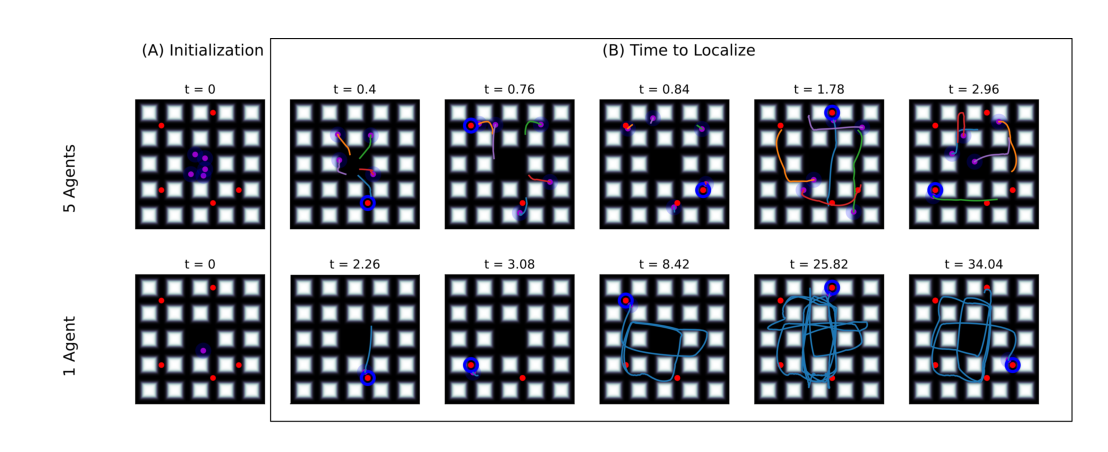
\includegraphics[scale=0.9]{figures/distr_loc2.eps}
\caption{ Localization of 5 targets in an environment with obstacles is shown for a single agent and a 5 agent network shown in Fig.~\ref{fig:path}. Each time frame shown indicates when a new agent was discovered in the environment. (A) The starting frame $t=0$ shows the starting location of each agent. Note that the 5 agent network distributes exploration amongst the agents which results in finding all 5 targets within $3$ seconds. Interestingly, ergodic exploration of 1 agent eventually results in the localization of all 5 agents given enough time to explore the environment. A monte-carlo simulation of the network localizing sequentially randomly generated targets is provided in the link: https://vimeo.com/209261679/0d65c1a9ac .}
\label{fig:disloc}
\end{figure*}

\subsection{Localization}

Results for localization are presented with the task to localize 5 targets within an environment with obstacles (see Fig.~\ref{fig:disloc}). Targets are shown as a red dot and initialized in the same way for a network of 1 agent and 5 agents. Each time an agent is localized, a blue circle is drawn at the time of localization from the initial starting point (Fig.~\ref{fig:disloc}). Each agent is not allowed to traverse the grey obstacles in the environment. Results show a clear benefit of utilizing consensus within ergodic exploration. Specifically, each individual agent explores their own particular subset of the environment. Therefore, each individual agent travels less which improves the overall energetic cost of moving while localizing all the targets at a much faster rate than with a single agent. The longer travel times are clearly noted in the trajectory traces of the single robot agent localizing the targets. Although the single agent requires longer time to localize all the targets, the ergodic control still successfully synthesizes actions that enable a single agent to span a large enough region to eventually localize all the targets.

The analysis of the localization example is furthered with a detailed observation of the ergodic measure. Figure~\ref{fig:disloc_conv} shows the convergence of the ergodic metric for the single agent, the collective 5 agent network, and the individual measures of ergodicity for each agent in the 5 agent network. With more agents, the ergodic measure reduces rapidly and is maintained in a non zero equilibrium value (this is due to the measure never being able to reach zero). The individual robotic agents ergodicity measures show similarity with the single agent network. Thus, regardless if consensus is reached, each agent will reduce the ergodic measure at their own particular rate. As consensus is reached, the rate of decent of the ergodic metric increases. When information about where each agent has explored is transferred through the network, the individual efforts result in an overall reduction in the ergodic metric.

\begin{figure}[!h]
\centering
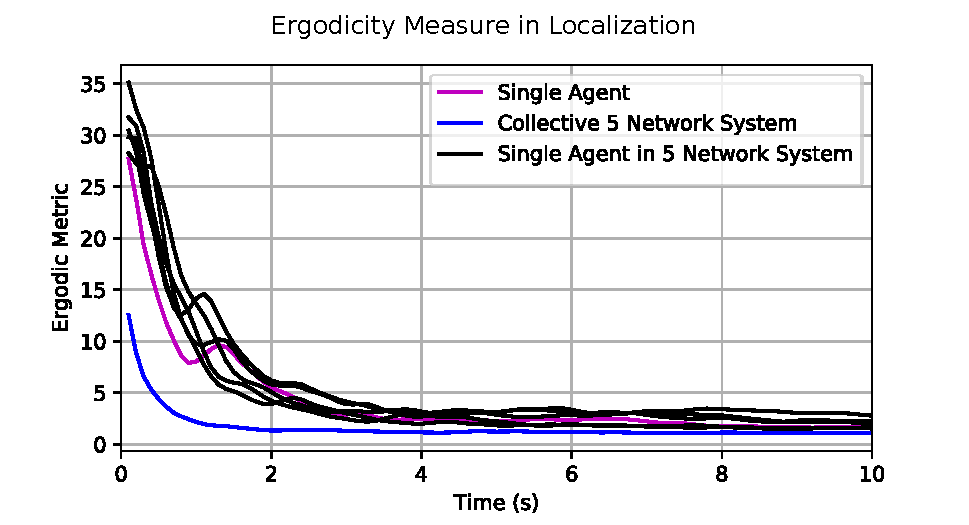
\includegraphics[scale=0.5]{figures/localization_convergence.pdf}
\caption{ Ergodicity measures for a single agent localizing 5 targets versus a 5 agent network localizing 5 targets. Each individual agent's ergodic measure is shown for the 5 agent network. Compared with the single agent, most robots individually have similar ergodic measures. As a connected network utilizing consensus, the ergodic measure is shown to be significantly less. This is due to shared information between agents on where each agent has been, thus each agent explores in a manner that is best for the collective group. }
\label{fig:disloc_conv}
\end{figure}

\subsection{Estimation}


Results for the problem of estimation is presented for a network of 5 autonomous aircraft that is tasked to estimate the terrain of a square grid. The motion of each agent is subject to the dynamics given by
\begin{equation*}
\begin{bmatrix}
\dot{x}  \\
\dot{y} \\
\dot{z} \\
\dot{\theta} \\
\dot{\psi}
\end{bmatrix} =
\begin{bmatrix}
u \cos(\theta) \cos(\psi) \\
u \cos(\theta) \sin(\psi) \\
u \sin(\theta) \\
v \\
w
\end{bmatrix}
\end{equation*}
where $(u,v,w)$ are the control inputs and $u > 0$ such that the aircraft must always be in motion. Each individual agent then takes measurements of the terrain height with which they are currently above\footnote{Each agent has an additional penalty to maintain a specific height above the terrain which prevents collision of the terrain.}. A distributed Kalman filter is used to estimate the terrain height based on the assumption that the terrain can be described as a network of radial-basis functions (RBFs) \cite{du2014radial}. RBFs are typically used to described a continuous surface using a discrete set of radial-basis functions. In this application, the RBFs are used as an estimator which can be used to generate an expected information density. As each agent acquires data, the distributed Kalman filter updates the terrain estimate and then forms a consensus on the estimate based on the network of the agents. The distributed ergodic control then synthesizes control actions that reduce the ergodic metric with respect to the expected information density.

\begin{figure*}[!th]
\centering
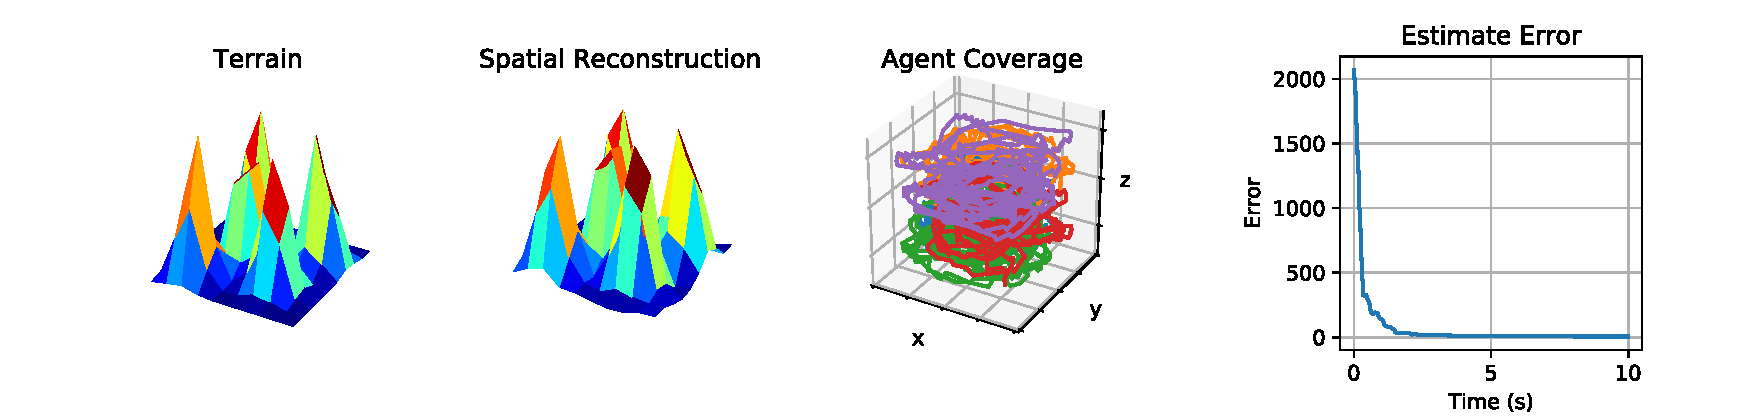
\includegraphics[scale=0.6]{figures/terrain_estimation.pdf}
\caption{ Terrain estimation is shown with a 5 agent aircraft network connected as shown in Fig.~\ref{fig:path}. Aircrafts take height measurements at each sampling rate and reconstruct the terrain based on a a radial-basis-function network. Agent coverage is shown to span the whole space. Estimate error is shown to provide a numerical measure of the accuracy of the spatial reconstruction.  }
\label{fig:estimation}
\end{figure*}

The ground truth terrain is shown in Fig.~\ref{fig:estimation} as well as the estimate for the 5 agent network after 10 second simulation time. For the alloted time, the estimate is shown to converge closely to the ground truth terrain. Although the graph connectivity is not that of a complete graph (a ring graph is used Fig.~\ref{fig:path}), the agent's coverage is still shown to grasp a significant amount of the allotted space for which the aircraft is allowed to travel.

\section{Conclusion} \label{sec:conc}

In this work, ergodic control is formulated as a means to synthesize actions that exhibit exploratory coverage behavior subject to a target statistical distribution. The formulation is then extended into a centralized distributed control problem for active exploration. Using graph theory and distributed optimization, ergodic control is reformulated in a completely distributed manner where information about past exploration is shared amongst agents. The sharing of past exploration provides a consensus on what has been explored and the sensitivity to the next action for each individual agent that reduces the ergodic metric. Various examples that utilize variants of ergodic control problem formulation are used to show improved convergence with additional agents, faster localization time and coverage, and rapid estimation of terrain.

In future work, we will examine the effects of the consensus matrix on the distributed ergodic control and augmentations to the controller to maintain network connectivity for time-varying graph topology.



\section*{Acknowledgments}

%% Use plainnat to work nicely with natbib.

\bibliographystyle{plainnat}
\bibliography{references}
\balance

\end{document}
